\chapter{Background}
\label{ch:background}

% (TODO): Re-read a lot of papers. Look for pieces of knowledge that are not
% included, but definitely should be.

Related work and the state of the art were reviewed, and identification of
relevant background material was carried out in the project preceding this
thesis \cite{aven_exploring_2019}. This background is herein amended with deeper
insights into the paradigm of physical reservoir computing, and adapted to fit a
thesis rather than an article. Specifically, the main focus is transferred from
physical limitations in general, to the narrower scope of spatial limitations
relating to physical morphology and topology.

\section{Complexity: Order, Chaos and Criticality}
\label{sec:criticality}

In deeming a physical system able to \textit{compute}, one implies information
storage, retrieval and modification. We are as humans intimately familiar with
the continuous, yet spontaneous computation present in our brains -- our
consciousness. We are less acquainted, however, with the conditions that
\textit{caused} the emergence of such a system.

Spanning a wide range of topics and disciplines, the field of \textit{complexity
theory} seeks answers to this conundrum. An exact definition of ``complexity''
is perhaps ever so elusive, but at its core lies an emergence of behavior
greater than the sum of its parts. Simple, local interactions give rise to
intricate, global patterns. This spontaneous emergence of complex behavior is
ubiquitous in nature. Ranging from convection cells in physics, to swarm and
flock behavior in biology, there is an abundance of interesting phenomena to
study \cite{heylighen_science_1999-1}.

Langton investigated the emergence of computation in cellular automata (CA)
\cite{langton_computation_1990}. His findings indicate a \textit{criticality} as
a condition to support computation. In essence, in between \textit{ordered} and
\textit{chaotic} dynamics, we find a critical phase transition. It is these
systems, intertwining order and chaos, that are of interest.

In systems that are too static, perturbation will fade too quickly. Chaotic
systems, on the other hand, are wildly unpredictable, making them excessively
sensitive. This \textit{edge of chaos} is a recurring theme in the investigation
of the computational capabilities of physical systems. In fact, the edge of
chaos has been found to be of significant in predicting the computational
performance of for neural microcircuit models, consisting of spiking neurons and
dynamic synapses \cite{legenstein_edge_2007}.

Biologically inspired models, most famously the artificial neural network (ANN),
are valuable scientific tools. Oftentimes, finding a suitable set of parameters
for a model will amount to much the same as finding the critical phase
transition between order and chaos. Reservoir computing (RC), a niche framework
within the field of machine learning, is concerned with observing the inherent
dynamics of a ``reservoir'' of local interconnections. Often employing random
neural networks, RC exploits the intrinsic computation emerging from these local
interconnections to solve practical tasks.

\section{Reservoir Computing Fundamentals}

% (TODO): Cite "Reservoir Computing as a Model for In-Materio Computing''

Training recurrent neural networks (RNN) is an inherently difficult
task. Gradient descent methods that incorporate loss information become
increasingly inefficient on problems with long-range temporal dependencies. This
inefficiency makes the backpropagation algorithm used with feed-forward
structures less attractive. Specifically, a continuous search in the parameter
space of recurrent networks may cause bifurcations points in the dynamics of the
system, causing non-convergent training \cite{doya_bifurcations_nodate}. To
circumvent this complexity, alternative methods that leave internal weights
untrained have been proposed.

Liquid state machines (LSMs) \cite{maass_real-time_2002} and echo state networks
(ESNs) \cite{jaeger_echo_2001} independently present supervised learning methods
that do not adapt the internal weights of the RNN. Instead, the output is
generated using a simple, memoryless classifier or regressor. This makes the RNN
function much like a kernel in kernel method algorithms, which seeks features
and general relations in datasets to increase separability.

Thus, by projecting into a high-dimensional space, temporal information of an
input may be incorporated in an instantaneous readout. This methodology has been
unified into the research subfield of RC \cite{schrauwen_overview_2007}, in
which the focus is on separating the randomly generated \textit{reservoir} from
the trained readout layer.

Interestingly, there is no need for the reservoir to be an artificial neural
network -- any high-dimensional, driven system exhibiting complex dynamic
behavior can be used \cite{schrauwen_overview_2007}. As long as the dynamics of
the \textit{substrate} can respond suitably to input, it can in theory be used
as a reservoir.

A multitude of substrates have shown promise as reservoirs: dynamical systems
models such as CA \cite{yilmaz_reservoir_2014}, and the more general random
Boolean network (RBN) \cite{snyder_computational_2013}, provide a discrete
alternative to the analogue ESN. Furthermore, a recent surge in physical
reservoir implementations has reinvigorated the field, which is introduced
further in Section \ref{sec:prc}.

\section{Echo State Networks}

\begin{figure}[t!]
  \centering
  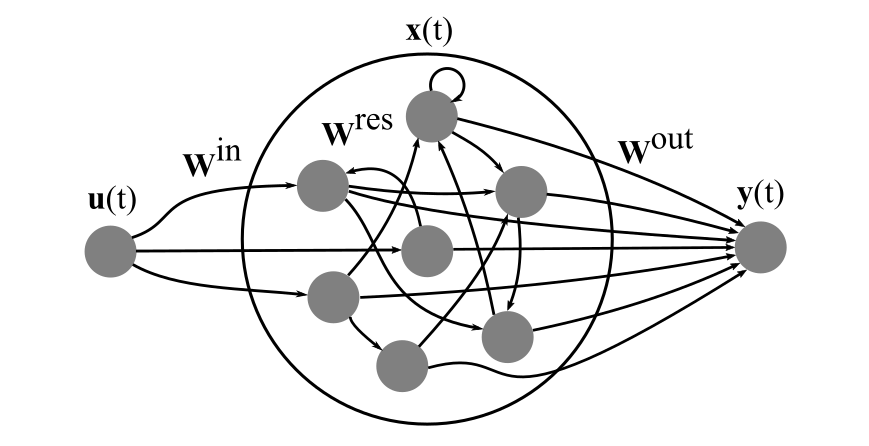
\includegraphics[width=3.0in]{figures/esn.png}
  \caption{
    Fig. 1: Basic architecture of ESN reservoir systems. The reservoir acts as a
high-dimensional kernel, transforming the temporal input sequence into a spatial
representation. The readout is trained with supervised linear regression,
providing a least squares optimum.
  }
  \label{fig:esn}
\end{figure}

The ESN is one of the key flavors of RC, and at its core lie untrained, randomly
initialized RNNs. Its conception introduced a highly practical approach to
training RNNs that is both simple and computationally feasible. In ESNs inner
weights remain fixed, and only the output weights are adapted to construct a
linear readout. The basic architecture of the ESN model is illustrated in Figure
\ref{fig:esn}, and it consists primarily of real-valued neurons connected by
unrestricted synapses, which results in a recurrent network.

\subsection{Echo State Network Internals}

% (TODO): Ask about re-using figures and text. Should be fine as it is cited and
% specified. Rephrasing is a stupid waste of time.

At time-step $t$, the ESN reservoir is defined by its input, internal, and
output units, denoted by $\mathbf{u}(t)$, $\mathbf{x}(t)$, and $\mathbf{y}(t)$,
respectively. The reservoir dynamics are characterized by three weight matrices,
$\mathbf{W}^{in}$, $\mathbf{W}^{res}$, and $\mathbf{W}^{out}$. In the
traditional ESN approach, the reservoir state is evolved according to

\begin{equation}
  \mathbf{x}(t + 1) =
    \tanh(\mathbf{W}^{res}\mathbf{x}(t)
        + \mathbf{W}^{in}\mathbf{u}(t)),
  \label{xt}
\end{equation}

\noindent using $\tanh$ as the nonlinear transfer function for internal
reservoir nodes. The output of the reservoir is given by

\begin{equation}
  \mathbf{y}(t) =
    \mathbf{W}^{out}\mathbf{x}(t).
  \label{yt}
\end{equation}

\subsection{Training}

To train an ESN model of size N in a supervised and offline mode, it is run to
completion on a training set. The reservoir states are collected row-wise into a
matrix $\mathbf{X}$, and the one-dimensional output into a vector
$\mathbf{Y}$. The linear readout layer is then trained to minimize the squared
output error $E = \norm{\mathbf{Y} - \mathbf{\hat{Y}}}$ where $\mathbf{\hat{Y}}$
is the target output, which amounts to finding the $\mathbf{W}^{out}$ that
minimizes the error with linear regression. Well-known methods include ridge
regression, often called Tikhonov regularization, and the Moore-Penrose
pseudo-inverse.

When the network is adapted to $\mathbf{W}^{out}$, the ESN is fully trained,
thus illustrating the apparent simplicity and low algorithmic complexity of the
method. Gauging the performance of a trained network is done by running a test
set.

\subsection{ESN Generation}

As with virtually every machine learning technique, the application of ESNs
requires some experience. Although a conceptually simple idea, generating
adequate reservoir networks is influenced by multiple global
parameters. Recommendations to achieve sufficient performance are presented in
\cite{montavon_practical_2012, jaeger_tutorial_2002}, suggesting parameters such
as the scaling of the input weight matrix $\boldsymbol{\iota}$, the spectral
radius of the reservoir connection matrix $\boldsymbol{\rho}$, and the model
size parameters to be of high importance. However, in practice the evaluation of
a reservoir is an endeavor often conducted by training the output and measuring
the error, sometimes requiring extensive parameter sweeps.

\textcolor{red}{
  Echo State Property and short-term memory. What does ``echo'' really mean? In
practice amounts mostly to input scaling and spectral radius. This is the memory
nonlinearity trade-off.
}

\textcolor{blue}{
  ``For the ESN approach to work, the reservoir should satisfy the so-called
echo state property: the state of the reservoir x(n) should be uniquely defined
by the fading history of the input u(n) [16]. In other words, for a long enough
input u(n), the reservoir state x(n) should not depend on the initial conditions
that were before the input.'' from practical guide to esn.
}

\subsection{Improvements to the Traditional ESN}

Many improvements have been made to the vanilla ESN, most of which are beyond
the scope of this thesis and its focus on physical reservoir
computing. Nevertheless, an introduction to the methodology would be incomplete
without a mention of some of the alterations that improve upon it.

Jaeger also proposed sigmoid reservoir nodes with memory to learn slow,
continuous dynamics \cite{jaeger_echo_2001}. In reservoirs with \textit{leaky
integrator neurons}, the nodes will not discard their previous state entirely,
but maintain a memory due to a leaking rate $\alpha$. Another addition proposed
by Jaeger is inserting noise into the training procedure, as it is well known in
the field of traditional artificial neural networks that an addition of noise to
training data can lead to generalization improvements similar to that of
Tikhonov regularization \cite{bishop_training_1995}.

Other important discoveries include improving reservoirs using intrinsic
plasticity \cite{schrauwen_improving_2008} and lateral inhibition
\cite{xue_decoupled_2007}, both inspired by concepts of neurobiology.

Lastly, stacking layers similarly to deep learning methods has been
attempted. With the aim of developing and enhancing \textit{hierarchical}
dynamics, it is intended to allow for multiple time-scales, and increased
richness in the reservoir, and has shown great promise
\cite{gallicchio_deep_2017}.

\subsection{Real World Applications}

The ESN methodology has been applied somewhat successfully to real world
tasks. Approaches include equalizing a wireless communication channel
\cite{jaeger_harnessing_2004}, and short-term traffic \cite{an_short-term_2011},
electric load \cite{song_hourly_2011}, and stock price forecasting
\cite{lin_short-term_2009}. Robot control is also a popular area of research for
RC applications, particularly for motor control and event detection
\cite{aislan_antonelo_learning_2015, harding_evolution_2005,
hutchison_movement_2004}. Perhaps less conventionally, RC has also been applied
in the context of reinforcement learning \cite{bush_modeling_2005}.

However, as the practicality of the paradigm resides primarily in chaotic time
series prediction and classification, this is also its main focus. Furthermore,
recent years have seen an increase in the realization of physical reservoirs to
accompany existing software simulations. An example is a silicon photonics chip
capable of 5-bit header recognition up to 12.5 Gbits$^{-1}$, and is scalable to
even higher bitrates \cite{vandoorne_experimental_2014}. This surge of optimism
has breathed new life into the field of RC, as physical reservoirs pave the way
for new types of integrated chips.

\subsection{Comparison to State of the Art}

Few definitive comparisons between the ESN and similar flavors of the RNN have
been carried out. The long short-term memory (LSTM) \cite{hochreiter_long_1997},
as well as its more recent descendant, the gated recurrent unit (GRU)
\cite{cho_learning_2014}, are mainstays in sequence processing, particularly in
natural language processing. Early experiments demonstrated the ESN methodology
to outperform previous LSTM methods on learning a chaotic attractor by orders of
magnitude \cite{jaeger_echo_2001}, but ESNs have largely remained a secondary
tool outside of chaotic time series prediction and classification.

A recent study compares the promising deep echo state network architecture
(DeepESN) to that of gated RNNs, where an experimental comparison between
recurrent models on multivariate time-series prediction tasks is made
\cite{gallicchio_comparison_2019}. It is established that the DeepESN
methodology outperforms other RNN approaches in their prediction ability on
challenging, real world datasets. The computation time is also lessened about
one order of magnitude compared to fully-trained RNN approaches. Thus, the
adoption of LSTM and GRU in practice may not necessarily be based on performance
suitability, but rather software availability and popularity.

\section{Assessing Reservoir Quality}
\label{sec:benchmark}

Designing \textit{good} reservoirs, possessing some set of desired properties,
naturally requires some metric by which we can evaluate and compare. Parameter
sweeps, i.e. our trial and error methods, must be accompanied by sufficient
methods of assessing computational performance.

Evaluation of reservoir quality is split into two different
approaches. Intuitively, measuring the performance of the model on a given
benchmark task is a simple, direct way of assessment. However, to gain an
intuition for a more general, expected performance across multiple benchmarks,
one may measure independent properties of the system, e.g. the spectral radius
of the internal weight matrix. The two approaches are often used in conjunction,
combined to propose an overall quality.

\subsection{Independent Metrics}
\label{ssec:metrics}

\subsubsection{Kernel Quality and Generalization}

Within the RC paradigm we are concerned with producing a complex mapping from
the input stream to some spatial, internal representation, such that a
memory-less, linear readout map may be employed for classification.

The \textit{linear separation property}, or \textit{kernel quality}, measures
ability to separate different inputs \cite{legenstein_edge_2007}. It is an
empirical measure of this complex mapping, denoting the potential diversity of
nonlinear operations carried out by a reservoir. Kernel quality is evaluated by
presenting a reservoir of size $n$ with $m$ different input sequences, and
computing the rank of the resulting $m\times n$ matrix consisting of the
reservoir states resulting at some time step $t$ for the input stream
\cite{busing_connectivity_2010}.

Another metric accompanying the kernel quality is the \textit{generalization
capability} of the reservoir \cite{legenstein_edge_2007}. This metric addresses
ability to generalize already learned functions or filters to new, unseen input,
and is used as an estimation of the VC-dimension of the
reservoir. Generalization capability is evaluated with the same method as kernel
quality, but instead requires input streams that are similar, or belong to the
same class \cite{busing_connectivity_2010}.

A reservoir in the ordered regime will naturally exhibit low values on both
metrics, while both metrics will be high in a network in the chaotic
regime. Thus, in general, reservoirs exhibiting a high kernel quality and a low
generalization rank are desirable, and the difference between the two is
sometimes used as its own metric \cite{busing_connectivity_2010}.

\subsubsection{Short-Term Memory}

Short-term memory capacity was introduced as a quantitative measurement of
linear memory capacity in reservoirs \cite{jaeger_short_2002}. It is a way to
examine the fading memory present in the system, and is measured by attaching
output units to the reservoir, which each are trained to recall some time
delayed version of the input sequence. By measuring how much of the input each
output unit can recover, we can estimate the memory capacity $MC$ by summing
over all time delays. Jaeger defined this as

\begin{equation}
  MC =
  \sum_{k}^{\infty}MC_{k} =
  \frac
  {cov^2(u(t-k), y_k(t))}
  {\sigma^{2}(u(t))\sigma^{2}(y_{k}(t))}
  ,
  \label{stm-eq}
\end{equation}

where $MC$ in general is limited by the reservoir size $N$, such that $MC \leq
N$. High input retention is a desirable property, but an increase in memory
capacity through parameter tuning is often met with a decrease in complex
information processing, due to a universal trade-off between memory and
nonlinearity \cite{dambre_information_2012}.

% (TODO): Not entirely orthogonal from generalization (see Burkow).

\subsubsection{Memory-Nonlinearity Trade-off}

Experimentation with a wide range of reservoirs has indicated a crucial
interplay between the memory and nonlinearity properties in reservoir operation
\cite{verstraeten_memory_2010}. In fact, the interplay has been uncovered to be
a universal trade-off between depth of memory and nonlinear computation
performed by a dynamical system \cite{dambre_information_2012}.

Thus, analyzing the boundary between an ordered, static regime that provides
memory, and a chaotic, dynamic regime that provides processing, is of vital
importance in the design of reservoirs. Determining the required nonlinearity
for a task is not a simple task, and often benefits from intuition about
nonlinear dynamics. Empirically, it has been shown that the input scaling,
determining the nonlinearity of reservoir responses, and the spectral radius,
scaling the importance of previous states, are the main parameters for
optimization in ESNs, illustrating the significance of the trade-off
\cite{montavon_practical_2012}.

Further formalization of the trade-off has been conducted, accompanied by a
proposition of a mixture reservoir combining both linear and nonlinear
dynamics. Adding a ``pinch of linearity'' is cited to improve performance
considerably \cite{inubushi_reservoir_2017}.

\subsubsection{Further Metrics}

A handful of other methods to assess quality and criticality of reservoirs have
been adapted, including the Lyapunov exponent
\cite{verstraeten_experimental_2007}, the Jacobian of the reservoir
\cite{alippi_quantification_2009}, Fisher information
\cite{livi_determination_2018}, and a separation ratio
\cite{gibbons_unifying_2010}.

In summary, given the vast amount of methods for evaluation, choosing a set of
suitable metrics is a surmountable task. This is especially so, given that few
metrics are entirely orthogonal, and are can be found to strongly correlate in
the prediction of performance \cite{chrol-cannon_correlation_2014}.

\subsection{Benchmarks}

Employing benchmarks to measure the performance of reservoirs is a means to
directly capture performance on specific tasks. Myriads of benchmarks exist
within the field of time series prediction, generation, and classification. The
benchmark spectrum range from simple tasks, to complicated, highly dynamic and
autoregressive time series.

Simpler tasks include the XOR problem of which is not linearly separable
\cite{goos_pattern_2003}, and n-bit temporal density and parity
\cite{bertschinger_real-time_2004}. More complex tasks may range from
recognizing isolated digits in speech \cite{verstraeten_isolated_2005}, to
predicting time series, of which the most popular are the Mackey-Glass time
delay differential equation \cite{mackey_oscillation_1977}, and the nonlinear
autoregressive moving average, NARMA \cite{atiya_new_2000}. Further datasets,
such as the Santa Fe Laser, Hénon Map, IPIX Radar, and Sunspot series datasets
have also been used \cite{rodan_minimum_2011}.

\subsubsection{NARMA - Nonlinear Autoregressive Moving Average}

\begin{figure}[t!]
  \centering
  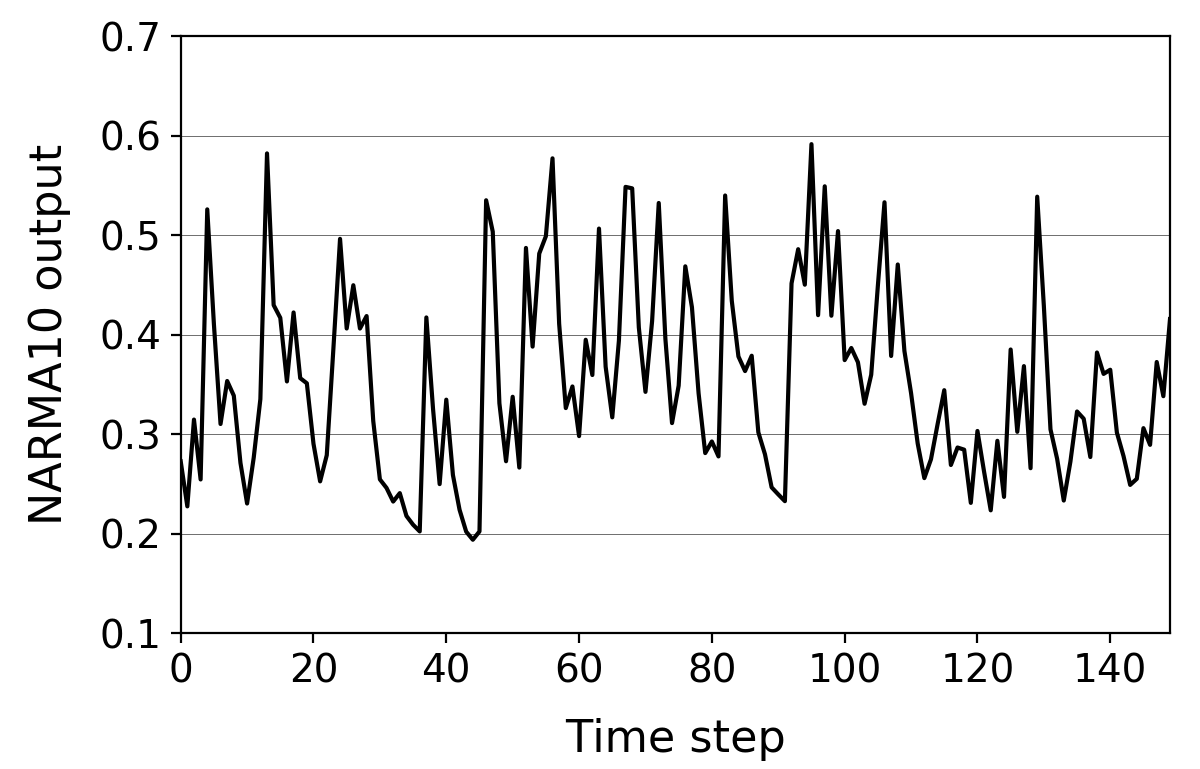
\includegraphics[width=3.0in]{figures/NARMA10.png}
  \caption{
    Example output generated by a 10th-order NARMA system. The autoregressive
moving average nature of the time series is clearly visible.
  }
  \label{fig:narma10}
\end{figure}

The class of time series provided by a nonlinear autoregressive moving average,
most often simply referred to as \textit{NARMA}, is a model commonly used to
benchmark recurrent networks \cite{atiya_new_2000}. Its widespread use yields
baseline performances for well established models, as well as more novel
approaches \cite{verstraeten_experimental_2007, appeltant_information_2011}. A
10th-order NARMA system is depicted in Figure \ref{fig:narma10}.

NARMA provides discrete-time temporal tasks, introducing a time-lag of $n$ time
steps, and is given by

\begin{equation}
  y_{t} = \alpha y_{t-1} +
  \beta y_{t-1} \sum_{i=1}^{n}y_{t-i} +
  \gamma u_{t-1}u_{t-n} +
  \delta
  .
  \label{eq:narma}
\end{equation}

Here, $n$ is the order of the system, and common constant parameters are $\alpha
= 0.3$, $\beta = 0.05$, $\gamma = 1.5$ and $\delta = 0.1$. The input $u_{t}$ is
an i.i.d. stream drawn uniformly from the interval [0, 0.5], and the nonlinear
product on the input sequence is shown in Figure
\ref{fig:narma-nonlinearity}. The time series is unstable, and tasks with higher
than a 10th-order time lag introduce a saturation function to produce a bounded
sequence:

\begin{equation}
  y_{t} =
  \tanh(
  \alpha y_{t-1} +
  \beta y_{t-1} \sum_{i=1}^{n}y_{t-i} +
  \gamma u_{t-1}u_{t-n} +
  \delta
  )
  .
  \label{eq:narma-tanh}
\end{equation}

\begin{figure}[t!]
  \centering
  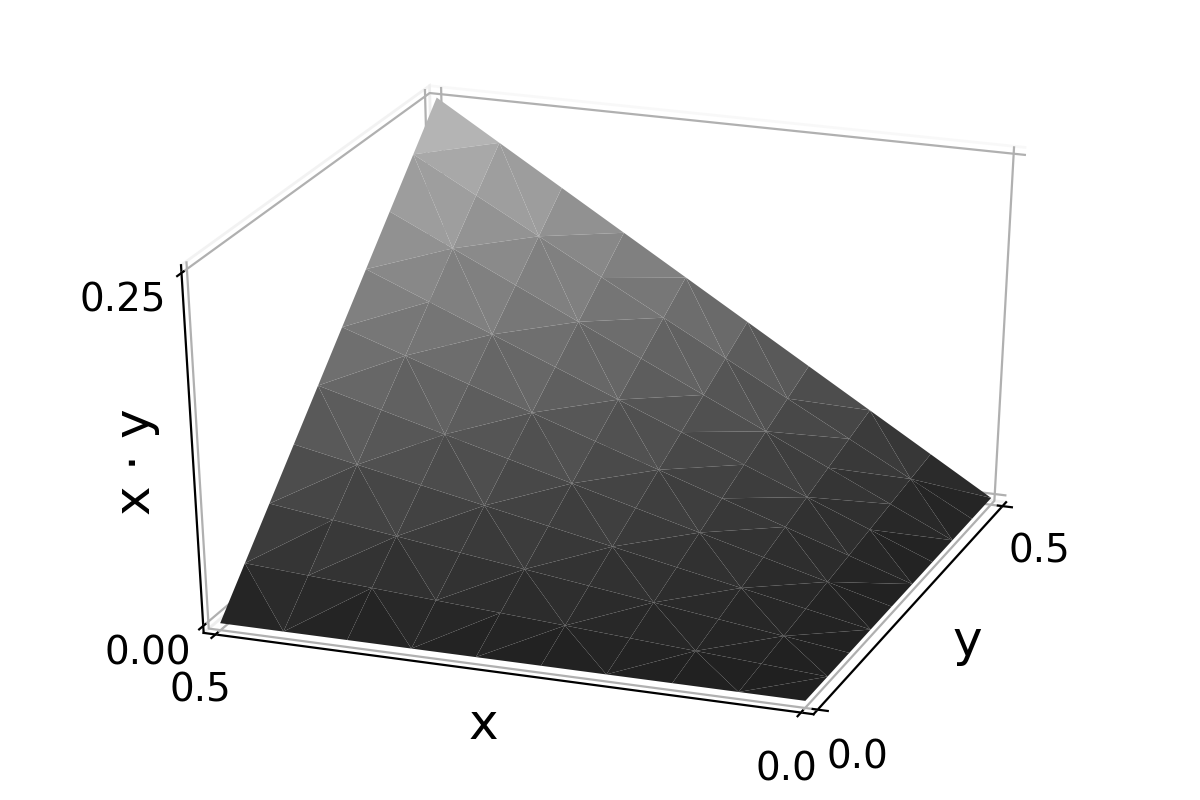
\includegraphics[width=3.0in]{figures/NARMA-nonlinearity.png}
  \caption{
    Nonlinear mapping of the product $u_{t-1}u_{t-n}$ of inputs in the NARMA
time series in Equation \protect\ref{eq:narma}.
  }
  \label{fig:narma-nonlinearity}
\end{figure}

Predicting a NARMA time series, given an input sequence $u$, presents a
challenge of both memory and nonlinearity. This makes NARMA well-suited for
evaluating both the memory capacity and computational power of reservoirs with a
single metric. Reservoirs must necessarily remember input sequences of length
$n$, and should preferably adhere to suitable dynamics on top of this.

Evaluation of ESN performance on the NARMA10 system is a thoroughly explored
area in the field of RC. Reported NRMSE performances for traditional ESN
reservoirs of size $N = 200$ lie in the range [0.20, 0.25]
\cite{verstraeten_experimental_2007, rodan_minimum_2011,
goudarzi_comparative_2014, jaeger_adaptive_2003}. For some context, using a
shift register containing the input as a reservoir will achieve a minimal NRMSE
of 0.4. To achieve NRMSE values below this threshold it is necessary to
introduce nonlinearity in the reservoir.

\subsubsection{Mackey-Glass Equation}

A common benchmark for dynamical systems is chaotic attractor learning. One such
benchmark is the Mackey-Glass delay differential equation

\begin{equation}
  \dot{y}(t) =
    \alpha \frac
    {y(t-\tau)}
    {1 + y(t-\tau)^\beta}
    - \gamma y(t),
  \label{eq:mg17}
\end{equation}

\begin{figure}[t!]
  \centering
  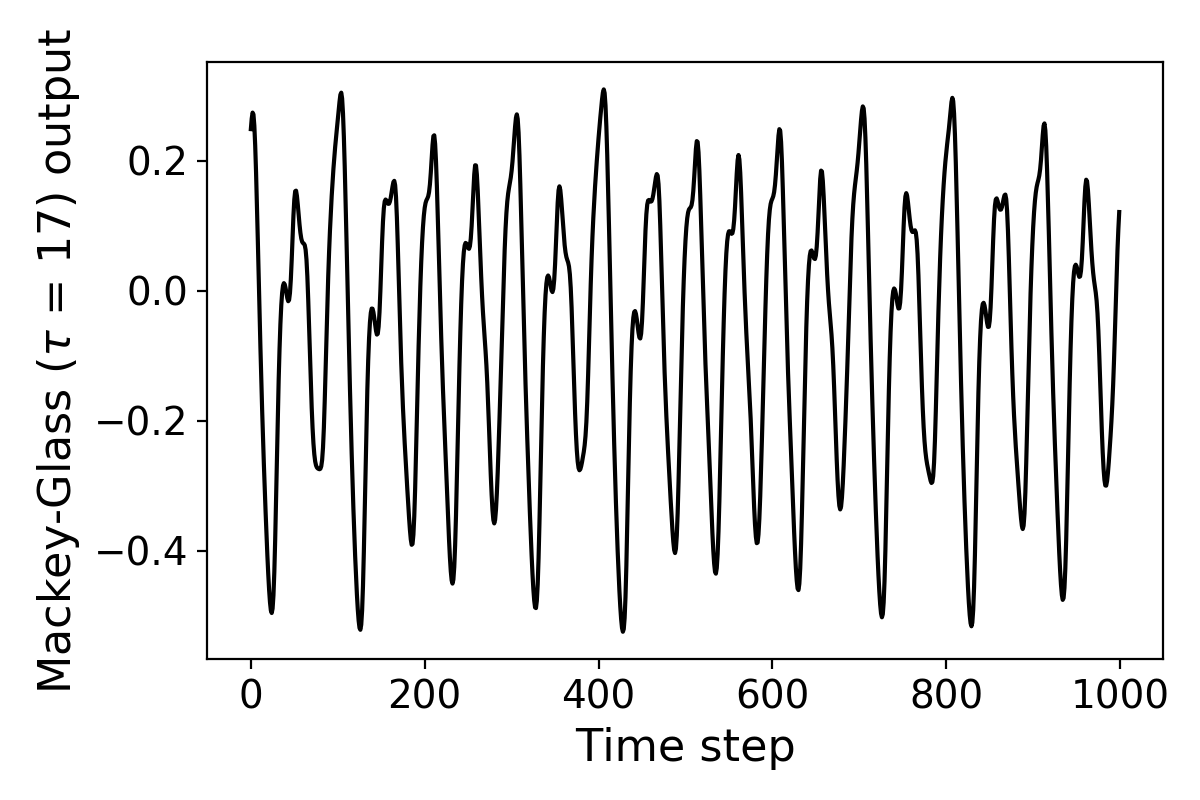
\includegraphics[width=3.0in]{figures/mg17-example.png}
  \caption{
    Sample sequence from the Mackey-Glass ($\tau = 17$) delay differential
equation.
  }
  \label{fig:mg17-example}
\end{figure}

where common constant parameters are $\alpha = 0.2$, $\beta = 10$ and $\gamma =
0.1$. A chaotic attractor appears when $\tau > 16.8$, and in practice $\tau =
17$ is used to generate a mildly chaotic attractor, while $\tau = 30$ yields
strongly chaotic behavior. The time series is most often generated with
numerical methods such as the Runge-Kutta method. Figure \ref{fig:mg17-example}
shows an example Mackey-Glass sequence with $\tau = 17$.

\section{Physical Reservoir Computing}
\label{sec:prc}

Developments in the field of RC have inevitably lead to novel and creative
approaches to reservoir design. Previously considered an ``exotic'' technique,
using physical substrates to realize reservoirs has become a common concept, and
the number of studies has been increasing rapidly. Physical reservoir computing
deviates from the traditional computer architecture in which processing and
memory units are separate entities, and into the territory of unconventional
computing. The notion of physical RC thus takes part in the evolution \textit{in
materio} paradigm \cite{miller_evolution_2002}, encompassing the general idea of
exploiting the physical properties of materials.

\subsection{Physical Reservoir Requirements}
\label{ssec:physreq}

What types of physical properties must be considered when experimenting with
novel materials for computation? Dale et al. suggest four key factors of
relevance: observability, nonlinear dynamics, methods of modeling the system,
and the impact of environmental factors \cite{adamatzky_reservoir_2017}. Tanaka
et al. present four requirements for physical reservoirs to efficiently solve
tasks: high dimensionality, nonlinearity, fading memory, and the separation
property \cite{tanaka_recent_2018}.

Hence, the computational requirements of physical reservoirs are similar to
those of conventional reservoirs. Their main difference lie in their
operability, as physical reservoirs tend to be harder to interact with. Suitable
input and output schemes must exist, and may be hindered by environmental
factors. Moreover, physical reservoirs have to be realized in a real, physical
space, which is further introduced in Section
\ref{ssec:topology-and-spatial-networks}.

In practice, physical reservoirs have been realized with a broad range of
substrates: photonic systems \cite{vandoorne_experimental_2014}, electronic
memristor circuits \cite{kulkarni_memristor-based_2012}, mechanical springs
\cite{hauser_towards_2011}, and more biologically oriented reservoirs such as
gene regulation networks \cite{jones_is_2007}, and the cat primary visual cortex
\cite{scholkopf_temporal_2007}. Consult \cite{tanaka_recent_2018} for a thorough
review of investigated physical substrates, their applications, and the general
trends in physical RC.

\subsection{Topology and Spatial Networks}
\label{ssec:topology-and-spatial-networks}

When designing physical reservoirs, there is a chance that the choice of
underlying topology is limited by physical factors, such as the type of physical
interactions that are present in the substrate. Additionally, physical
reservoirs must necessarily be embedded in physical space. The layout of
vertices and edges of such systems, however complicated their dynamics may be,
are thus \textit{restricted by space}. Topology alone proves insufficient to
describe these networks, as these spatial constraints determine freedom in
structure, i.e. node position and edge cost.

The real world presents us with plenty of networks that possess spatial
components, ranging from the Internet to rail roads. Models have been developed
to study the properties of these networks, which in turn may be useful in
studying reservoirs that will have spatial constraints imposed. Enticing models
include the Watts-Strogatz model \cite{watts_collective_1998}, with its
small-world properties, and the Waxman model \cite{waxman_routing_1988}, where
nodes are connected with a probability that depends on the distance between
them. A thorough review of spatial networks is presented in
\cite{barthelemy_spatial_2011}.

However, in the context of physical reservoir computing, it may turn out to be
helpful to take a step back. Before delving for interesting spatial models, it
is important to gain insight into the performance penalties one might expect
from enforcing a spatial layout in the first place. The foundation of the ESN is
the Erdos-Renyi graph \cite{erdos_random_1959}, a simple model for random
geometric graphs in which nodes are connected with a probability $p$. Imposing a
metric space onto the ESN model, in practice a bare minimum, allows us to
observe the simplest spatial reservoir.

\subsubsection{Related Work}

Rodan and Tiňo discovered that simple, cyclic reservoirs, i.e. ring topologies,
perform comparably to the ESN \cite{rodan_minimum_2011}. These cyclic reservoirs
were later extended with regular jumps to consistently outperform regular ESNs
\cite{rodan_simple_2012}. Gallicchio et al. reported similar findings in their
work on DeepESN, where structured schemes such as multiple rings lead to the
best performances \cite{gallicchio_reservoir_2019}.

Dale et al. compared ring, lattice, and fully-connected reservoir topologies
\cite{mcquillan_role_2019}.  They argue that fully-connected ESNs exhibit the
highest substrate quality, given higher memory capacities and a better ability
to produce rich nonlinear representation of the input. The discrepancy between
performance predicted by these metrics and the benchmarks used by Rodan and Tiňo
in their work on ring topologies should be noted.

Lastly, Manevitz et al. have found small world topologies to produce fault
tolerant reservoirs \cite{sidorov_stability_2010}. Errors resulting from
introducing dead and noisy neurons were remedied by choosing a connectivity
scheme pertaining to a power law distribution, illustrating superiority to
uniform connectivity in terms of robustness.

Research on reservoir computing with constrained topology or physical morphology
is a relatively sparse area. There is much to be discovered about the impact of
reservoir construction with structured organization. Moreover, efforts to find
useful topologies should also yield valuable insights about why the stochastic
ESN works so well, to allow for more deterministic construction of reservoirs
with desirable properties.

%%% Local Variables:
%%% mode: latex
%%% TeX-master: "../thesis"
%%% End: